\documentclass[a4paper, 11pt, oneside]{article}

\newcommand{\plogo}{\fbox{$\mathcal{PL}$}} 
\usepackage{amsmath}
\usepackage[utf8]{inputenc} 
\usepackage[T1]{fontenc} 
\usepackage{enumitem}
\usepackage{graphicx}
\usepackage{graphicx}
\usepackage{supertabular}
\usepackage[spanish]{babel}
\graphicspath{{Imagenes/}}

\begin{document} 

\begin{titlepage} 

	\centering 
	
	\scshape 
	
	\vspace*{\baselineskip} 
	
	
	
	\rule{\textwidth}{1.6pt}\vspace*{-\baselineskip}\vspace*{2pt} 
	\rule{\textwidth}{0.4pt} 
	
	\vspace{0.75\baselineskip} 
	
	{\LARGE Resumen 11: GRUB}	
	\vspace{0.75\baselineskip} 
	
	\rule{\textwidth}{0.4pt}\vspace*{-\baselineskip}\vspace{3.2pt}
	\rule{\textwidth}{1.6pt} 
	
	\vspace{2\baselineskip} 
	

	ADMINISTRACIÓN DE SISTEMAS UNIX/LINUX
	
	\vspace*{3\baselineskip} 
	
	
	
	Alumna:
	
	\vspace{0.5\baselineskip} 
	
	{\scshape\Large Karla Adriana Esquivel Guzmán \\} 
	\vspace{0.5\baselineskip} 
	\vfill
	
\includegraphics{unam.jpg}
	
	\textit{UNIVERSIDAD NACIONAL AUTONOMA DE MEXICO} 
	
	\vfill
	
	
	
	
	\vspace{0.3\baselineskip} 
	
	12/Febrero/2019 
	
	 

\end{titlepage}
\section*{Definición de GRUB:}

Es el primer software que se ejecuta en la computadora después del BIOS. Su misión es cargar el kernel de un sistema operativo, en pocas palabras es un gestor de arranque. 

\section*{GRUB2:}
En fedora tenemos por default a GRUB2(Grand Unified Bootloader 2). GRUB2 además es compatible con todos los sistemas operativos, incluido Windows, todas las distribuciones de Linux y casi todos los sistemas operativos similares a Unix, como macOS.\\
En el directorio \textbf{etc/\ grub.d} están almacenados los archivos de configuración y los scripts de instalación, pueden modificarse, sin embargo hay que ser cuidadosos y contar con un respaldo. Aunque GRUB2 fue simplemente definida en clase como un gestor/cargador que permite poner contraseñas y también permite navegar en otros sistemas operativos.
En Ubuntu el directorio \textbf{/\ boot/\ grub} contiene el archivo \textbf{grub.cfg} este es el conjunto principal de archivos de configuración para grub.cfg se encuentra en el directorio $/etc/grub.d$. Cada uno de los archivos en ese directorio contiene el código GRUB que se recopila en el archivo grub.cfg final. El esquema de numeración utilizado en los nombres de estos archivos de configuración está diseñado para proporcionar el pedido de modo que el archivo grub.cfg final se reúna en la secuencia correcta. Cada uno de estos archivos tiene un comentario para indicar el principio y el final de la sección, y esos comentarios también forman parte del archivo grub.cfg, de modo que es posible ver desde qué archivo se genera cada sección.

\begin{center}
 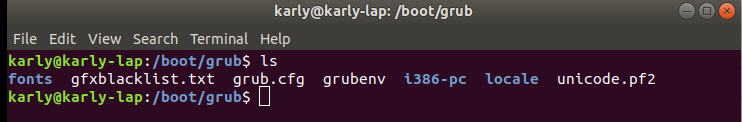
\includegraphics[scale=0.20]{11202.png}
\end{center}
Utilizando el comando cat para abrir el archivo de texto plano \textbf{grub.cfg}  y podremos ver lo ya mencionado anteriormente.

\begin{center}
 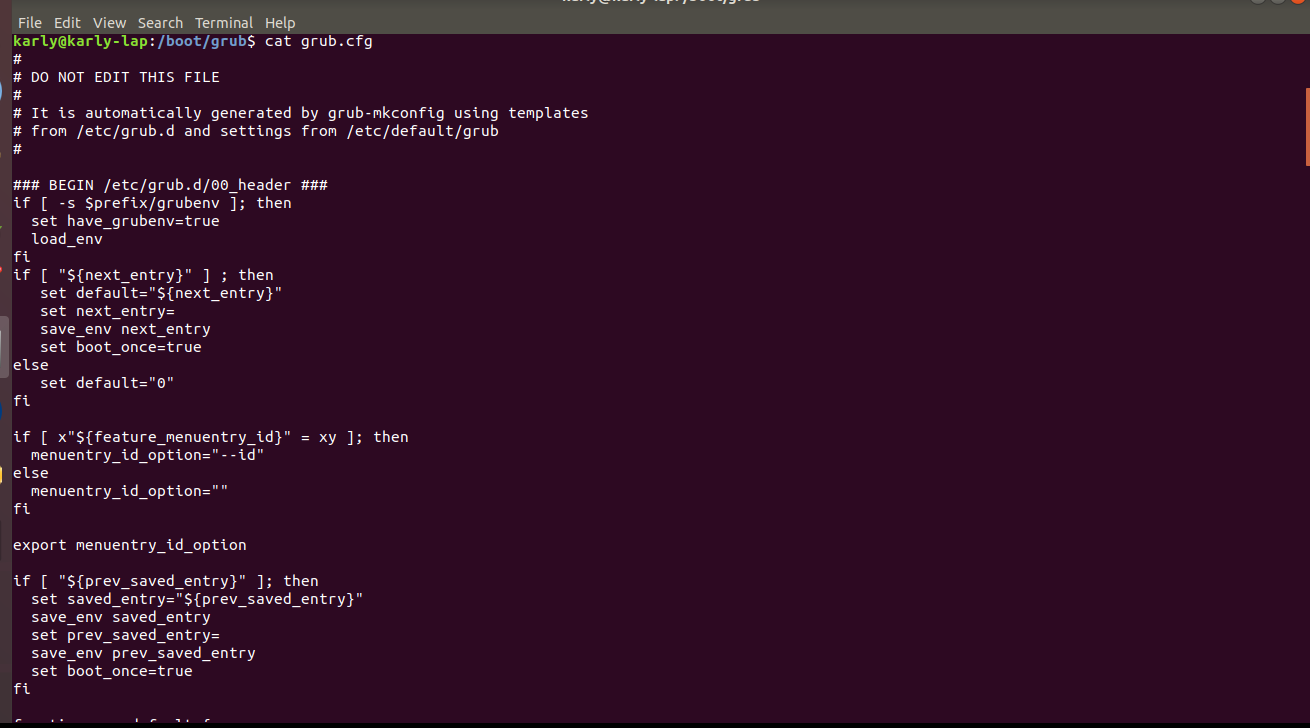
\includegraphics[scale=0.20]{21202.png}
\end{center}


\end{document}
